\documentclass[11pt]{article}
\usepackage[a4paper,margin=21mm]{geometry}
\usepackage{amsmath,amssymb,booktabs,array}
\usepackage{tikz}
\usepackage[T1]{fontenc}
\usepackage{lmodern}
\usepackage[hidelinks]{hyperref}
\usepackage{listings}
\lstset{basicstyle=\ttfamily\small,breaklines=true,columns=fullflexible,frame=single}
\setlength{\parindent}{0pt}
\setlength{\parskip}{6pt}
\newcommand{\mos}[4]{\begin{scope}[shift={(#1,#2)}]
\draw (0,.24)--(0,-.24);
\draw (0,.20)--(.25,.20)--(.25,.5);
\draw (0,-.20)--(.25,-.20)--(.25,-.5);
\draw (-.16,.23)--(-.16,-.23);
\ifnum#4=1\draw (-.26,0) circle (.06);\draw (-.75,0)--(-.32,0);\else\draw (-.75,0)--(-.16,0);\fi
\node[anchor=east,font=\small] at (-.76,0) {$#3$};
\end{scope}}
\newcommand{\ground}[2]{\draw (#1,#2)--(#1,{#2-.12});\draw ({#1-.17},{#2-.12})--({#1+.17},{#2-.12});\draw ({#1-.11},{#2-.20})--({#1+.11},{#2-.20});}
\newcommand{\rail}[3]{\draw (#1,#2)--(#1,{#2+.15});\node[above,font=\small] at (#1,{#2+.15}) {$#3$};}
\newcommand{\outputnode}[3]{\fill (#1,#2) circle (.04);\draw (#1,#2)--({#1+.7},#2) node[right] {$#3$};}
\begin{document}
\begin{center}{\Large\bfseries Introduction to VLSI Design, 2020}\par{\large Homework 3: measured pre-layout AND-gate delays}\end{center}
\section*{Circuit and chosen dimensions}
The six-transistor circuit is a two-input NAND followed by an inverter. The assignment labels the internal NAND output \textbf{F} and the loaded AND output \textbf{Z}:
\[
 F=\overline{AB},\qquad Z=AB.
\]
The output capacitor is explicitly $C_L=1$ fF from Z to ground. All NMOS bodies connect to ground, including the upper transistor in the NAND stack; all PMOS bodies connect to $V_{DD}$.
\begin{center}\begin{tikzpicture}[scale=.94]
\mos{0}{2.5}{A}{1}\mos{2}{2.5}{B}{1}\draw (.25,3)--(2.25,3);\rail{1.25}{3}{V_{DD}}
\draw (.25,2)--(2.25,2);\fill (2.25,2) circle (.04);\node[below] at (2.7,2){$F$};
\mos{0}{1.5}{A}{0}\mos{0}{.5}{B}{0}\ground{.25}{0}
\draw (2.25,2)--(3.8,2);\draw (3.8,1)--(3.8,2.5);\draw (3.8,1)--(4.75,1);\draw (3.8,2.5)--(4.75,2.5);
\mos{5.5}{2.5}{}{1}\mos{5.5}{1}{}{0}\draw (5.75,1.5)--(5.75,2);\rail{5.75}{3}{V_{DD}}\ground{5.75}{.5}\outputnode{5.75}{1.75}{Z}
\draw (6.5,1.75)--(6.5,1.25);\draw (6.25,1.25)--(6.75,1.25);\draw (6.25,1.1)--(6.75,1.1);\draw (6.5,1.1)--(6.5,.7);\ground{6.5}{.7}\node[right,font=\small] at (6.85,1.18){1 fF};
\end{tikzpicture}\end{center}
\begin{center}\begin{tabular}{lrr}\toprule Device&$W$ ($\mu$m)&$L$ ($\mu$m)\\\midrule
NAND PMOS A, B&2.50&0.18\\NAND NMOS A, B&2.00&0.18\\Inverter PMOS&2.50&0.18\\Inverter NMOS&1.00&0.18\\\bottomrule\end{tabular}\end{center}
Doubling each NAND NMOS width approximately compensates its two-device series path relative to the inverter NMOS. PMOS width is an arbitrary reasonable choice allowed by the prompt, not an optimization claim. The included diffusion area/perimeter estimates assume a $0.18\,\mu$m extension for every source/drain. They are declared schematic estimates rather than layout extraction. The sum of channel areas is $2.25\,\mu\mathrm{m}^2$.

\section*{Simulation and delay convention}
HSPICE S-2021.09 uses the local CIC018 \texttt{N\_18/P\_18} TT models at 1.8 V and 25 C. Inputs settle for 2 ns, then each changing input ramps over 20 ps. The primary transient output interval and maximum solver step are 1 ps. A separate copy is used for each transition, avoiding ambiguity from mixed pulse trains. Propagation delay is measured from the changing input's $0.5V_{DD}=0.9$ V crossing to the target node's 0.9 V crossing. For simultaneous A/B changes, their crossings coincide, so either input is a valid trigger.

All six output-changing transitions are required: $00,01,10\to11$ and their reverses. The remaining six directed transitions among the four input words do not change the settled AND/NAND output and have no steady-state propagation delay to report. A hazard on those transitions would be a different measurement. Separate worst cases are selected for each node and each output direction.
\newpage\section*{Measured results}
The following values are actual HSPICE measurements with 20 ps input slew. Output directions are measured at F and Z, not copied from the direction of an input.
\begin{center}\begin{tabular}{lccrr}\toprule Input transition&F direction&Z direction&F delay (ps)&Z delay (ps)\\\midrule
$00\to 11$&HL&LH&29.4932&47.6815\\
$01\to 11$&HL&LH&23.0762&41.2842\\
$10\to 11$&HL&LH&29.1938&47.3766\\
$11\to 00$&LH&HL&19.2001&38.2918\\
$11\to 01$&LH&HL&30.9294&52.1393\\
$11\to 10$&LH&HL&41.8569&63.7000\\
\bottomrule\end{tabular}\end{center}
\begin{center}\begin{tabular}{lclr}\toprule Node&Output direction&Worst transition&Worst delay (ps)\\\midrule
F&HL&\texttt{00->11}&29.4932\\
F&LH&\texttt{11->10}&41.8569\\
Z&HL&\texttt{11->10}&63.7000\\
Z&LH&\texttt{00->11}&47.6815\\
\bottomrule\end{tabular}\end{center}
The F low-to-high delay depends on which PMOS charges F and on the internal stack node's state. F high-to-low depends on discharging through the two-device stack; simultaneous rises must establish conduction through both devices. Z's delay includes the F transition followed by the inverter response, so its worst case can differ from F's.

\section*{Numerical checks and input-slew dependence}
All simulated before/after levels passed the voltage limits: $V_H\ge1.6$ V and $V_L\le0.2$ V. Per-run evidence is saved in \path{level_checks.csv}. Tightening the maximum step from 1 ps to 0.2 ps changed the delay by at most $0.128958$ ps; see \texttt{convergence.csv}. This checks numerical resolution without claiming unlimited precision in the underlying models.

A second sweep with 1 ns input ramps is saved in \texttt{delays.csv}. Slower ramps alter delay substantially; propagation delay is meaningful only with its input slew, load, supply, sizes, model corner, and threshold convention specified. The report's headline worst cases use the declared 20 ps slew.
\newpage\section*{Measured waveform examples}
The traces below are sampled simulator voltages, drawn directly in this standalone LaTeX source. Time zero is the input's 50-percent crossing; the horizontal dotted line is the 0.9 V delay threshold. The first example produces the largest F fall and Z rise delays. The second produces the largest F rise and Z fall delays.
\begin{center}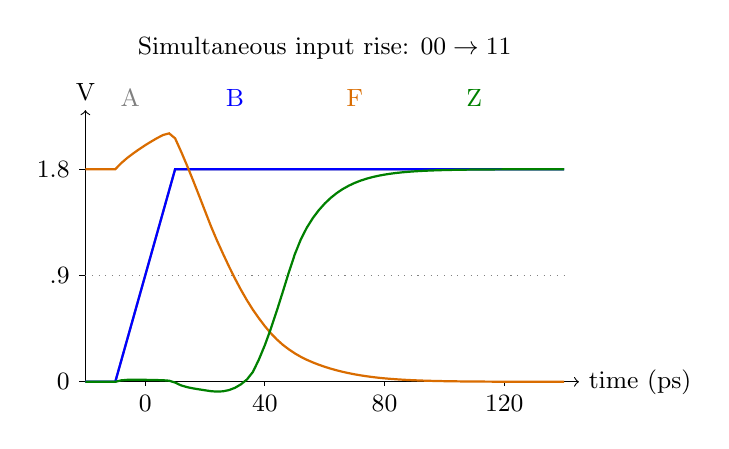
\begin{tikzpicture}[x=.038cm,y=1.5cm]
\draw[->] (0,0)--(165,0) node[right,font=\small]{time (ps)};
\draw[->] (0,0)--(0,2.3) node[above,font=\small]{V};
\draw[dotted,gray] (0,.9)--(160,.9);
\foreach \x/\t in {20/0,60/40,100/80,140/120}{\draw (\x,0)--(\x,-.035) node[below,font=\small]{$\t$};}
\foreach \y in {0,.9,1.8}{\draw (0,\y)--(-2,\y) node[left,font=\small]{$\y$};}
\draw[gray,thick] plot coordinates {(0.000,0.000000) (2.000,0.000000) (4.000,0.000000) (6.000,0.000000) (8.000,0.000000) (10.000,0.000000) (12.000,0.180000) (14.000,0.360000) (16.000,0.540000) (18.000,0.720000) (20.000,0.900000) (22.000,1.080000) (24.000,1.260000) (26.000,1.440000) (28.000,1.620000) (30.000,1.800000) (32.000,1.800000) (34.000,1.800000) (36.000,1.800000) (38.000,1.800000) (40.000,1.800000) (42.000,1.800000) (44.000,1.800000) (46.000,1.800000) (48.000,1.800000) (50.000,1.800000) (52.000,1.800000) (54.000,1.800000) (56.000,1.800000) (58.000,1.800000) (60.000,1.800000) (62.000,1.800000) (64.000,1.800000) (66.000,1.800000) (68.000,1.800000) (70.000,1.800000) (72.000,1.800000) (74.000,1.800000) (76.000,1.800000) (78.000,1.800000) (80.000,1.800000) (82.000,1.800000) (84.000,1.800000) (86.000,1.800000) (88.000,1.800000) (90.000,1.800000) (92.000,1.800000) (94.000,1.800000) (96.000,1.800000) (98.000,1.800000) (100.000,1.800000) (102.000,1.800000) (104.000,1.800000) (106.000,1.800000) (108.000,1.800000) (110.000,1.800000) (112.000,1.800000) (114.000,1.800000) (116.000,1.800000) (118.000,1.800000) (120.000,1.800000) (122.000,1.800000) (124.000,1.800000) (126.000,1.800000) (128.000,1.800000) (130.000,1.800000) (132.000,1.800000) (134.000,1.800000) (136.000,1.800000) (138.000,1.800000) (140.000,1.800000) (142.000,1.800000) (144.000,1.800000) (146.000,1.800000) (148.000,1.800000) (150.000,1.800000) (152.000,1.800000) (154.000,1.800000) (156.000,1.800000) (158.000,1.800000) (160.000,1.800000)};
\draw[blue,thick] plot coordinates {(0.000,0.000000) (2.000,0.000000) (4.000,0.000000) (6.000,0.000000) (8.000,0.000000) (10.000,0.000000) (12.000,0.180000) (14.000,0.360000) (16.000,0.540000) (18.000,0.720000) (20.000,0.900000) (22.000,1.080000) (24.000,1.260000) (26.000,1.440000) (28.000,1.620000) (30.000,1.800000) (32.000,1.800000) (34.000,1.800000) (36.000,1.800000) (38.000,1.800000) (40.000,1.800000) (42.000,1.800000) (44.000,1.800000) (46.000,1.800000) (48.000,1.800000) (50.000,1.800000) (52.000,1.800000) (54.000,1.800000) (56.000,1.800000) (58.000,1.800000) (60.000,1.800000) (62.000,1.800000) (64.000,1.800000) (66.000,1.800000) (68.000,1.800000) (70.000,1.800000) (72.000,1.800000) (74.000,1.800000) (76.000,1.800000) (78.000,1.800000) (80.000,1.800000) (82.000,1.800000) (84.000,1.800000) (86.000,1.800000) (88.000,1.800000) (90.000,1.800000) (92.000,1.800000) (94.000,1.800000) (96.000,1.800000) (98.000,1.800000) (100.000,1.800000) (102.000,1.800000) (104.000,1.800000) (106.000,1.800000) (108.000,1.800000) (110.000,1.800000) (112.000,1.800000) (114.000,1.800000) (116.000,1.800000) (118.000,1.800000) (120.000,1.800000) (122.000,1.800000) (124.000,1.800000) (126.000,1.800000) (128.000,1.800000) (130.000,1.800000) (132.000,1.800000) (134.000,1.800000) (136.000,1.800000) (138.000,1.800000) (140.000,1.800000) (142.000,1.800000) (144.000,1.800000) (146.000,1.800000) (148.000,1.800000) (150.000,1.800000) (152.000,1.800000) (154.000,1.800000) (156.000,1.800000) (158.000,1.800000) (160.000,1.800000)};
\draw[orange!85!black,thick] plot coordinates {(0.000,1.800000) (2.000,1.800000) (4.000,1.800000) (6.000,1.800000) (8.000,1.800000) (10.000,1.800000) (12.000,1.851887) (14.000,1.895502) (16.000,1.933825) (18.000,1.969433) (20.000,2.003149) (22.000,2.034122) (24.000,2.063595) (26.000,2.089781) (28.000,2.103383) (30.000,2.061170) (32.000,1.949402) (34.000,1.830124) (36.000,1.705365) (38.000,1.576819) (40.000,1.446030) (42.000,1.315738) (44.000,1.196154) (46.000,1.084671) (48.000,0.976971) (50.000,0.874455) (52.000,0.778873) (54.000,0.690793) (56.000,0.610014) (58.000,0.537882) (60.000,0.470885) (62.000,0.411107) (64.000,0.358764) (66.000,0.313283) (68.000,0.275043) (70.000,0.240909) (72.000,0.211755) (74.000,0.186617) (76.000,0.164497) (78.000,0.144801) (80.000,0.127173) (82.000,0.111373) (84.000,0.097226) (86.000,0.084594) (88.000,0.073356) (90.000,0.063404) (92.000,0.054631) (94.000,0.046933) (96.000,0.040211) (98.000,0.034365) (100.000,0.029303) (102.000,0.024935) (104.000,0.021180) (106.000,0.017960) (108.000,0.015208) (110.000,0.012861) (112.000,0.010863) (114.000,0.009167) (116.000,0.007728) (118.000,0.006510) (120.000,0.005480) (122.000,0.004610) (124.000,0.003877) (126.000,0.003258) (128.000,0.002737) (130.000,0.002298) (132.000,0.001929) (134.000,0.001619) (136.000,0.001359) (138.000,0.001140) (140.000,0.000956) (142.000,0.000801) (144.000,0.000672) (146.000,0.000563) (148.000,0.000472) (150.000,0.000396) (152.000,0.000332) (154.000,0.000278) (156.000,0.000233) (158.000,0.000195) (160.000,0.000163)};
\draw[green!50!black,thick] plot coordinates {(0.000,0.000000) (2.000,0.000000) (4.000,0.000000) (6.000,0.000000) (8.000,0.000000) (10.000,0.000000) (12.000,0.012279) (14.000,0.016786) (16.000,0.017732) (18.000,0.017453) (20.000,0.016763) (22.000,0.015703) (24.000,0.014660) (26.000,0.013255) (28.000,0.009324) (30.000,-0.006526) (32.000,-0.030430) (34.000,-0.045116) (36.000,-0.055505) (38.000,-0.063902) (40.000,-0.071859) (42.000,-0.079475) (44.000,-0.082948) (46.000,-0.080385) (48.000,-0.070207) (50.000,-0.050874) (52.000,-0.021451) (54.000,0.019473) (56.000,0.083505) (58.000,0.188470) (60.000,0.310707) (62.000,0.449731) (64.000,0.601795) (66.000,0.762480) (68.000,0.925869) (70.000,1.078895) (72.000,1.204994) (74.000,1.304104) (76.000,1.384775) (78.000,1.452156) (80.000,1.508966) (82.000,1.556933) (84.000,1.597359) (86.000,1.631326) (88.000,1.659776) (90.000,1.683534) (92.000,1.703326) (94.000,1.719782) (96.000,1.733444) (98.000,1.744776) (100.000,1.754168) (102.000,1.761951) (104.000,1.768399) (106.000,1.773743) (108.000,1.778173) (110.000,1.781847) (112.000,1.784894) (114.000,1.787424) (116.000,1.789526) (118.000,1.791272) (120.000,1.792724) (122.000,1.793932) (124.000,1.794938) (126.000,1.795775) (128.000,1.796473) (130.000,1.797055) (132.000,1.797540) (134.000,1.797945) (136.000,1.798282) (138.000,1.798564) (140.000,1.798800) (142.000,1.798996) (144.000,1.799160) (146.000,1.799298) (148.000,1.799413) (150.000,1.799508) (152.000,1.799589) (154.000,1.799656) (156.000,1.799712) (158.000,1.799759) (160.000,1.799798)};
\node[above,font=\small] at (80,2.65){Simultaneous input rise: $00\to11$};
\node[font=\small,text=gray] at (15,2.4){A};\node[font=\small,text=blue] at (50,2.4){B};
\node[font=\small,text=orange!85!black] at (90,2.4){F};\node[font=\small,text=green!50!black] at (130,2.4){Z};
\end{tikzpicture}\end{center}
\begin{center}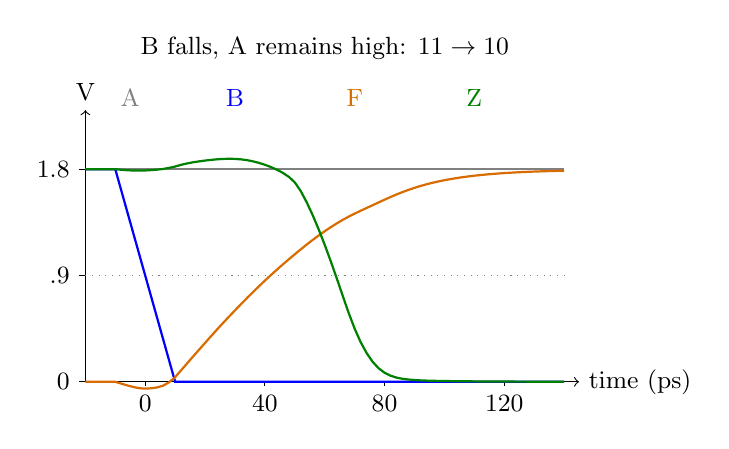
\begin{tikzpicture}[x=.038cm,y=1.5cm]
\draw[->] (0,0)--(165,0) node[right,font=\small]{time (ps)};
\draw[->] (0,0)--(0,2.3) node[above,font=\small]{V};
\draw[dotted,gray] (0,.9)--(160,.9);
\foreach \x/\t in {20/0,60/40,100/80,140/120}{\draw (\x,0)--(\x,-.035) node[below,font=\small]{$\t$};}
\foreach \y in {0,.9,1.8}{\draw (0,\y)--(-2,\y) node[left,font=\small]{$\y$};}
\draw[gray,thick] plot coordinates {(0.000,1.800000) (2.000,1.800000) (4.000,1.800000) (6.000,1.800000) (8.000,1.800000) (10.000,1.800000) (12.000,1.800000) (14.000,1.800000) (16.000,1.800000) (18.000,1.800000) (20.000,1.800000) (22.000,1.800000) (24.000,1.800000) (26.000,1.800000) (28.000,1.800000) (30.000,1.800000) (32.000,1.800000) (34.000,1.800000) (36.000,1.800000) (38.000,1.800000) (40.000,1.800000) (42.000,1.800000) (44.000,1.800000) (46.000,1.800000) (48.000,1.800000) (50.000,1.800000) (52.000,1.800000) (54.000,1.800000) (56.000,1.800000) (58.000,1.800000) (60.000,1.800000) (62.000,1.800000) (64.000,1.800000) (66.000,1.800000) (68.000,1.800000) (70.000,1.800000) (72.000,1.800000) (74.000,1.800000) (76.000,1.800000) (78.000,1.800000) (80.000,1.800000) (82.000,1.800000) (84.000,1.800000) (86.000,1.800000) (88.000,1.800000) (90.000,1.800000) (92.000,1.800000) (94.000,1.800000) (96.000,1.800000) (98.000,1.800000) (100.000,1.800000) (102.000,1.800000) (104.000,1.800000) (106.000,1.800000) (108.000,1.800000) (110.000,1.800000) (112.000,1.800000) (114.000,1.800000) (116.000,1.800000) (118.000,1.800000) (120.000,1.800000) (122.000,1.800000) (124.000,1.800000) (126.000,1.800000) (128.000,1.800000) (130.000,1.800000) (132.000,1.800000) (134.000,1.800000) (136.000,1.800000) (138.000,1.800000) (140.000,1.800000) (142.000,1.800000) (144.000,1.800000) (146.000,1.800000) (148.000,1.800000) (150.000,1.800000) (152.000,1.800000) (154.000,1.800000) (156.000,1.800000) (158.000,1.800000) (160.000,1.800000)};
\draw[blue,thick] plot coordinates {(0.000,1.800000) (2.000,1.800000) (4.000,1.800000) (6.000,1.800000) (8.000,1.800000) (10.000,1.800000) (12.000,1.620000) (14.000,1.440000) (16.000,1.260000) (18.000,1.080000) (20.000,0.900000) (22.000,0.720000) (24.000,0.540000) (26.000,0.360000) (28.000,0.180000) (30.000,0.000000) (32.000,0.000000) (34.000,0.000000) (36.000,0.000000) (38.000,0.000000) (40.000,0.000000) (42.000,0.000000) (44.000,0.000000) (46.000,0.000000) (48.000,0.000000) (50.000,0.000000) (52.000,0.000000) (54.000,0.000000) (56.000,0.000000) (58.000,0.000000) (60.000,0.000000) (62.000,0.000000) (64.000,0.000000) (66.000,0.000000) (68.000,0.000000) (70.000,0.000000) (72.000,0.000000) (74.000,0.000000) (76.000,0.000000) (78.000,0.000000) (80.000,0.000000) (82.000,0.000000) (84.000,0.000000) (86.000,0.000000) (88.000,0.000000) (90.000,0.000000) (92.000,0.000000) (94.000,0.000000) (96.000,0.000000) (98.000,0.000000) (100.000,0.000000) (102.000,0.000000) (104.000,0.000000) (106.000,0.000000) (108.000,0.000000) (110.000,0.000000) (112.000,0.000000) (114.000,0.000000) (116.000,0.000000) (118.000,0.000000) (120.000,0.000000) (122.000,0.000000) (124.000,0.000000) (126.000,0.000000) (128.000,0.000000) (130.000,0.000000) (132.000,0.000000) (134.000,0.000000) (136.000,0.000000) (138.000,0.000000) (140.000,0.000000) (142.000,0.000000) (144.000,0.000000) (146.000,0.000000) (148.000,0.000000) (150.000,0.000000) (152.000,0.000000) (154.000,0.000000) (156.000,0.000000) (158.000,0.000000) (160.000,0.000000)};
\draw[orange!85!black,thick] plot coordinates {(0.000,0.000000) (2.000,0.000000) (4.000,0.000000) (6.000,0.000000) (8.000,0.000000) (10.000,0.000000) (12.000,-0.015280) (14.000,-0.030324) (16.000,-0.043767) (18.000,-0.053975) (20.000,-0.057674) (22.000,-0.054960) (24.000,-0.047524) (26.000,-0.032685) (28.000,-0.003581) (30.000,0.038689) (32.000,0.097496) (34.000,0.155794) (36.000,0.213783) (38.000,0.271426) (40.000,0.328925) (42.000,0.386101) (44.000,0.442509) (46.000,0.497539) (48.000,0.551444) (50.000,0.604573) (52.000,0.656909) (54.000,0.708354) (56.000,0.758814) (58.000,0.808198) (60.000,0.856405) (62.000,0.903330) (64.000,0.948988) (66.000,0.993677) (68.000,1.037073) (70.000,1.079537) (72.000,1.121615) (74.000,1.162490) (76.000,1.201523) (78.000,1.238799) (80.000,1.274494) (82.000,1.308540) (84.000,1.340650) (86.000,1.370603) (88.000,1.398321) (90.000,1.423875) (92.000,1.447966) (94.000,1.471516) (96.000,1.494992) (98.000,1.518517) (100.000,1.541817) (102.000,1.564463) (104.000,1.586047) (106.000,1.606278) (108.000,1.625001) (110.000,1.642168) (112.000,1.657805) (114.000,1.671985) (116.000,1.684802) (118.000,1.696361) (120.000,1.706768) (122.000,1.716127) (124.000,1.724534) (126.000,1.732082) (128.000,1.738854) (130.000,1.744927) (132.000,1.750372) (134.000,1.755252) (136.000,1.759625) (138.000,1.763543) (140.000,1.767054) (142.000,1.770199) (144.000,1.773017) (146.000,1.775542) (148.000,1.777806) (150.000,1.779835) (152.000,1.781654) (154.000,1.783286) (156.000,1.784750) (158.000,1.786064) (160.000,1.787244)};
\draw[green!50!black,thick] plot coordinates {(0.000,1.800000) (2.000,1.800000) (4.000,1.800000) (6.000,1.800000) (8.000,1.800000) (10.000,1.800000) (12.000,1.795230) (14.000,1.791432) (16.000,1.788937) (18.000,1.788014) (20.000,1.789329) (22.000,1.792354) (24.000,1.796336) (26.000,1.801923) (28.000,1.811070) (30.000,1.822461) (32.000,1.837091) (34.000,1.848838) (36.000,1.858440) (38.000,1.866158) (40.000,1.873019) (42.000,1.878900) (44.000,1.883690) (46.000,1.886958) (48.000,1.888307) (50.000,1.887295) (52.000,1.883500) (54.000,1.876695) (56.000,1.866805) (58.000,1.853816) (60.000,1.837711) (62.000,1.818427) (64.000,1.795878) (66.000,1.769237) (68.000,1.735807) (70.000,1.688680) (72.000,1.614685) (74.000,1.519011) (76.000,1.409879) (78.000,1.289741) (80.000,1.160101) (82.000,1.022358) (84.000,0.878132) (86.000,0.730018) (88.000,0.584064) (90.000,0.451064) (92.000,0.336714) (94.000,0.244165) (96.000,0.169978) (98.000,0.115176) (100.000,0.077101) (102.000,0.051899) (104.000,0.035755) (106.000,0.025568) (108.000,0.019117) (110.000,0.014945) (112.000,0.012145) (114.000,0.010172) (116.000,0.008707) (118.000,0.007565) (120.000,0.006637) (122.000,0.005859) (124.000,0.005193) (126.000,0.004614) (128.000,0.004106) (130.000,0.003658) (132.000,0.003261) (134.000,0.002909) (136.000,0.002596) (138.000,0.002318) (140.000,0.002070) (142.000,0.001849) (144.000,0.001652) (146.000,0.001477) (148.000,0.001321) (150.000,0.001182) (152.000,0.001058) (154.000,0.000947) (156.000,0.000848) (158.000,0.000760) (160.000,0.000682)};
\node[above,font=\small] at (80,2.65){B falls, A remains high: $11\to10$};
\node[font=\small,text=gray] at (15,2.4){A};\node[font=\small,text=blue] at (50,2.4){B};
\node[font=\small,text=orange!85!black] at (90,2.4){F};\node[font=\small,text=green!50!black] at (130,2.4){Z};
\end{tikzpicture}\end{center}
The full six-transition voltage data, including the settled intervals, are available in \texttt{waveforms.csv}. These examples use only the 20 ps slew, 1 ps maximum-step measurements.
\newpage\section*{Reconciliation with previous submissions}
J.-M. Wu's \texttt{HW3 107501503} PDF includes a NAND/inverter and 1 fF load but drives the 1.8 V model devices at 3.3 V. Its upper NMOS body is tied to an internal stack node rather than the grounded substrate, and it tabulates only transitions into 11. The reported values (F: 251, 125, 153 ps; Z: 270, 142, 170 ps) are not treated as results for this corrected 1.8 V circuit.

S.-Y. Sun's \texttt{VLSI HW3.docx} uses 1.8 V and grounded NMOS bodies and discusses both output directions. However, the listed code omits the assigned 1 fF load and uses a coarse 0.1 ns transient interval. Its six-transistor topology is retained; this solution explicitly restores the load, measures all six transitions automatically, declares input slew and parasitics, sizes the NAND stack, and checks the timestep. Different simulations cannot be merged by choosing the smallest delay.

\section*{Reproduction}
Run the following command:
\begin{lstlisting}
python simulate.py --model D:/cic018.l --raw-dir <scratch>
\end{lstlisting}
Supply \texttt{--hspice <executable>} if necessary. The script generates 18 simulator runs (6 transitions at each of three slew/step settings), exports delays and level checks, and leaves raw listing/license metadata in the scratch directory. \texttt{testbench.sp} is the directly runnable primary $00\to11$ example; \texttt{and2.sp} is the reusable circuit. The process library and licenses are not part of the repository.

\end{document}
